
\section{Prepare data}
\label{sec:dataPrepare}
\subsection{Raw data}

Data should be prepared as the example in Figure~\ref{fig:dataMicroarray}.
First column should be feature ID (e.g. gene symbol) and the rest of the columns are samples.
Note that the first column can also be other feature type (i.e. probe id, entrez ID).
The first row is sample ID.
Valid data type includes continuous data and count data.

\begin{figure}[H]
\begin{center}
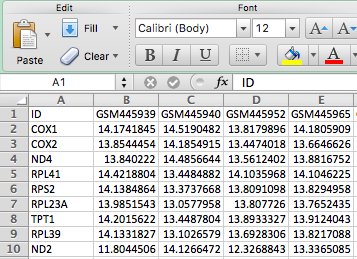
\includegraphics[scale=0.5]{./figure/dataPreparation/dataMicroarray}
\caption{A example input data format}
\label{fig:dataMicroarray}
\end{center}
\end{figure}

\subsection{Clinical data}

Clinical data should be prepared as the example in Figure~\ref{fig:clinical}.
First column should be sample ID and each row represents a sample.
The rest of the columns are clinical information (e.g. case/control labels).

\begin{figure}[H]
\begin{center}
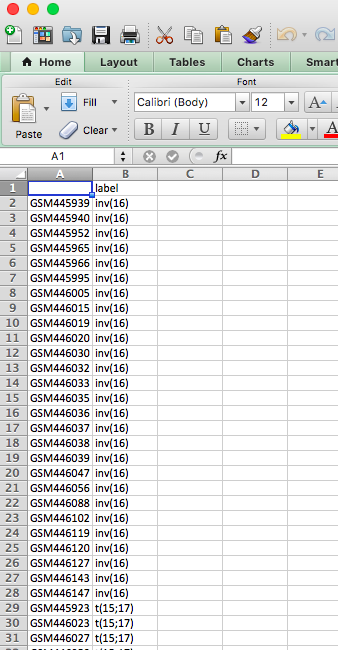
\includegraphics[scale=0.5]{./figure/dataPreparation/clinicalData}
\caption{A example clinical data format}
\label{fig:clinical}
\end{center}
\end{figure}

\subsection{Example data with the MetaOmics software}


We collected three multi-study examples as testing datasets for the MetaOmics software.
Table~\ref{tab:realDataLeukemia} shows three acute myeloid leukemia (AML) gene expression profiles.
Table~\ref{tab:realDataBreastCancer} shows four breast cancer gene expression profiles, in which the first study contains both count data and FPKM data.
Table~\ref{tab:realDataProstate} shows gene expression profiles from eight prostate cancer datasets.
The leukemia datasets are used to demonstrate MetaProcess, MetaDE, MetaPath, MetaNetwork, MetaPredict, MetaClust and MetaPCA.
The prostate cancer datasets are used to demonstrate MetaQC.

			\begin{table}[h]
			\caption{Multi-study acute myeloid leukemia (AML) gene expression profiles. All three studies are from Affymetrix Human Genome U133plus2 with 5,135 genes.
		Three subtypes of leukemia are defined as the chromosomal translocation,
		including inversion of chromosome 16 - inv(16), translocation of chromosome 15 and 17 - t(15:17) and 
		translocation of chromosome 8 and 21 - t(8:21).}						
			\centering
\begin{tabular}{c  c  c   c   }
  \hline 
  \hline 
\multirow{2}*{Study}   & \multirow{2}*{source}   & \multirow{2}*{\# samples}  & \# samples by subtypes \\
 & & & inv(16)/t(15:17)/t(8,21)  \\
  \hline 
Study 1 & \cite{verhaak2009prediction} & 89 & 33/21/35\\
Study 2 & \cite{balgobind2011evaluation} & 74 & 27/19/28\\
Study 3 & \cite{kohlmann2008international} & 105 & 28/37/40\\
  \hline 
  \hline 
\end{tabular}
			\label{tab:realDataLeukemia}
		\end{table}
		
			\begin{table}[h]
			\caption{Multi-study breast cancer gene expression profiles. 
			Each gene expression profiles of all four studies contain 10,330 genes.
			Study 1 contains both count data and fpkm (continuous) data so user should {\bf select only one of them}. 
			The other three studies contain only continuous data.
			The phenotype of interest is estrogen-receptor (comparing ER+ vs ER-).}						
			\centering
			\begin{tabular}{c  c  c   c  c  }
			  \hline 
			  \hline 
			\multirow{2}*{Study}   & \multirow{2}*{source}   & \multirow{2}*{scale}  & \multirow{2}*{\# samples}  & \# samples by ER \\
 & & & & ER+/ER-  \\
  \hline 
\multirow{2}*{Study 1}  & \multirow{2}*{\cite{weinstein2013cancer}}  & count & \multirow{2}*{406} & \multirow{2}*{319/87}\\
&& continuous && \\
Study 2 & \cite{desmedt2007strong} & continuous &  198 & 134/64\\
Study 3 & \cite{wang2005gene} & continuous & 286 & 209/77\\
Study 4 & \cite{ivshina2006genetic} & continuous & 245 & 211/34\\
  \hline 
  \hline 
\end{tabular}
			\label{tab:realDataBreastCancer}
		\end{table}


			\begin{table}[h]
			\caption{Multi-study prostate cancer dataset information. Eight prostate cancer gene expression profiles were measured by different microarray platforms.}						
			\centering
	\begin{tabular}{c c c c c}
	\hline
	\hline
\multirow{2}*{Study}   & \multirow{2}*{source}   & \multirow{2}*{\# samples}  & \# samples by label  & \multirow{2}*{\# genes}\\
& & & Normal/Primary& \\
	\hline
	Study 1 & \cite{welsh2001analysis} &  34 & 9/25 & 8798 \\
	Study 2 & \cite{yu2004gene} &  146 & 81/65 & 8799 \\
	Study 3 & \cite{lapointe2004gene} &  103 & 41/62 & 13579 \\
	Study 4 & \cite{varambally2005integrative} &  13 & 6/7 & 19738 \\
	Study 5 & \cite{singh2002gene}  &  102 & 50/52  & 8799 \\
	Study 6 & \cite{wallace2008tumor} &  89 & 20/69 & 12689  \\
	Study 7 & \cite{nanni2006epithelial} &  30 & 7/23  & 12689 \\
	Study 8 & \cite{tomlins2006tmprss2} &  57 & 27/30 & 9703   \\
	\hline
	\hline
	\label{tab:prostate}
	\end{tabular}
			\label{tab:realDataProstate}
		\end{table}



